\documentclass{article}

\usepackage[UTF8]{ctex}       %中文
\usepackage{microtype}        %排版相关
\usepackage[american]{babel}  %排版相关
\usepackage{amsmath}          %数学公式
\usepackage{amssymb}          %数学公式
\usepackage{url}
\usepackage{tikz}
\usepackage{gnuplot-lua-tikz}
\usepackage{graphicx}
\usepackage{caption}
\usepackage{float} 
\usepackage{subfigure}
%\usepackage{subcaption}
\usetikzlibrary{calc,positioning, shapes.geometric}
%\usepackage{cite}%引用
%\usepackage[numbers,sort&compress]{natbib}
\title{Finalwork:一维非线性方程的求解}
\author{Janice\_zh\quad 信息与计算科学 3200103473}
\date{\today} 

\begin{document}
	\maketitle   %加标题
	%\renewcommand{\contentsname}{目录}
	%\tableofcontents  %加目录
	
	\renewcommand{\abstractname}{摘要}
	\begin{abstract}
		本文介绍求解一维非线性方程$f(x)=0$的算法实现和技术要点。总体来说可将求解方法分为``root bracketing''和``root polishing''两类。我们将详细介绍二分法、牛顿法和Brent法的算法实现,并对其收敛性和收敛速度进行比较。然后我们将对不同的函数进行算例测试,探究求解一维非线性方程的技术要点。最后得出结论。\cite{R3}
	\end{abstract}
	\section{引言}
	对于一维低阶线性方程,我们易由公式法或其他方法很快得出方程的根。然而当阶数较高时,很难直接利用公式法求解,因此我们考虑利用迭代法实现对一维非线性方程的求解。
	\section{数学理论与技术要点}
	\paragraph{}目前求解一维非线性方程的方法可分为两类:第一种不断对解的可能区间进行迭代,称为``root bracketing'',如二分法,Brent法;第二种不断对一个近似解进行迭代,称为``root poshing'',如牛顿法。
	\paragraph{}不同的迭代方式在迭代算法实现上有所不同,但总体的迭代步骤一致,如下所示:
	\begin{verbatim}
	·对于算法T,初始化状态s
	·利用T对s进行迭代
	·判断s的收敛性,若未达到要求则重复迭代过程
	\end{verbatim}
	\paragraph{}
	不同的迭代方法对于初始状态的要求不同,但总体来说,初始可能区间、初始近似解、最大迭代次数、精度要求以及函数本身的性质都会影响迭代的效果。因此,对于一个给定的方程,可以利用图像等对方程的根进行大致预估,选取合适的解区间、近似解、求解方法以及上述的其他因素就成为了求解一维非线性方程的技术要点。
	\section{算法实现与收敛性比较}
	\subsection{算法实现}
	\subsubsection{二分法}
	\paragraph{}给定可能解区间,每次取中点二分进行迭代。是最简单的一种迭代方式,线性收敛。同时要求给定区间端点的函数值异号,且不能处理偶数重根的情况。\\
	%\begin{figure}
		%\centering
		\begin{tikzpicture}
		[node distance=10pt]
		\node[draw, rounded corners] (1) {给定方程$f(x)=0$和解的可能区间$[lo,hi]$,要求满足$f(lo)*f(hi)<0$};
		\node[draw, below=20pt of 1] (2) {取中点$mid=\frac{lo+hi}{2}$};
		\node[draw, diamond, aspect=2, below=of 2]  (3)  {f(lo)*f(mid)<0};
		\node[draw, left=30pt of 3] (4)  {hi=mid};
		\node[draw, right=30pt of 3] (5)  {lo=mid};
		\node[draw, below=20pt of 3] (8) {得到新区间[lo,hi]};
		\node[draw, diamond, aspect=2,below=20pt of 8] (6)  {判断是否达到要求};
		\node[draw, rounded corners, below=30pt of 6]  (7) {得到方程的根};
		
		\draw[->] (1) -- (2);
		\draw[->] (2) -- (3);
		\draw[->] (3) -- node[above]  {Yes}(4);
		\draw[->] (3) -- node[above]  {No}(5);
		\draw[->] (4) -- (8);
		\draw[->] (5) -- (8);
		\draw[->] (8) -- (6);
		\draw[->]  (6.east)--($(6.east)+(3,-0)$)--node[right]{No}($(2.east)+(3.5cm,0)$)-- (2.east);
		\draw[->] (6) -- node[right]  {Yes}(7);		
		\end{tikzpicture}
	%	\caption{二分法}
	%	\label{二分法_algo}
	%\end{figure}
	\subsubsection{牛顿法}
	\paragraph{}不断迭代近似解,切线与x轴的交点迭代成为新的近似解。单根二次收敛,复根线性收敛。求解效率与准确度比较依赖初始近似解的选取。(篇幅原因流程图在此不再赘述)
		%\begin{figure}
		%\centering
		%\begin{tikzpicture}
		%[node distance=10pt]
		%\node[draw, rounded corners] (1) {给定方程$f(x)=0$和近似解$x_0$, $i=0$};
		%\node[draw, below=20pt of 1] (2) {迭代:$x_{i+1}=x_i-\frac{f(x_i)}{f^{'}(x_i)}$,  i = i+1}; 
		%\node[draw, diamond, aspect=2,below=20pt of 2] (6)  {判断解$x_i$是否达到要求};
		%\node[draw, rounded corners, below=30pt of 6]  (4) {得到方程的根};
		
		%\draw[->] (1) -- (2);
		%\draw[->] (2) -- (3);
		%\draw[->] (3) -- (6);
		%\draw[->]  (6.east)--($(6.east)+(2,-0)$)--node[right]{No}($(2.east)+(1.85cm,0)$)-- (2.east);
		%\draw[->] (6) -- node[right]  {Yes}(4);		
		%\end{tikzpicture}
		%	\caption{牛顿法}
		%	\label{牛顿法_algo}
		%\end{figure}
		\subsubsection{secant法}
		\paragraph{}牛顿法的简化,从第二步开始用数值估计替代导数。多重根线性收敛。适合在根附近导数无明显变化的函数方程,依赖原方程的特点与初始近似解的选取。(篇幅原因无流程图)
			%\begin{figure}
			%\centering
			%\begin{tikzpicture}
			 
			%[node distance=10pt]
			%\node[draw, rounded corners] (1) {给定方程$f(x)=0$和近似解$x_0$, $i=0$};
			%\node[draw, below=20pt of 1] (8) %{$x_1=x_0-\frac{f(x_0)}{f^{'}(x_0)}$,  i = 1}; 
			%\node[draw, below=20pt of 8] (2) {迭代:$x_{i+1}=x_i-\frac{f(x_i)}{f^{'}_{est}}$ where$ f^{'}_{est}=\frac{f(x_i)-f(x_{i-1})}{x_i-x_{i-1}}$, $i = i+1$}; 
			%\node[draw, diamond, aspect=2,below=20pt of 2] (6)  {判断解$x_i$是否达到要求};
			%\node[draw, rounded corners, below=30pt of 6]  (4) {得到方程的根};
			
			%\draw[->] (1) -- (8);
			%\draw[->] (8) -- (2);
			%\draw[->] (2) -- (6);
			%\draw[->]  (6.east)--($(6.east)+(4,-0)$)--node[right]{No}($(2.east)+(1.8cm,0)$)-- (2.east);
			%\draw[->] (6) -- node[right]  {Yes}(4);		
			%\end{tikzpicture}
			%	\caption{secant法}
			%	\label{secant法_algo}
			%\end{figure}
	\subsection{收敛性比较}
	分别用二分法,牛顿法,secant法求解$x^2-5=0$。\cite{R2}
		
		\begin{figure}[ht]
			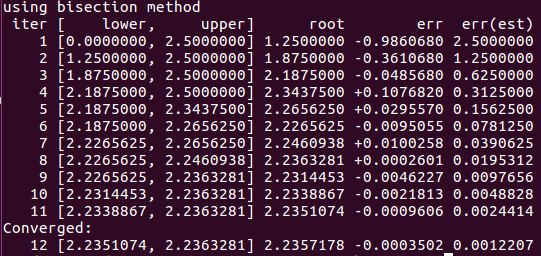
\includegraphics[width=1\linewidth]{images/bisection.png}
			%\caption{bisection}
		\end{figure}
			\begin{figure}[ht]
				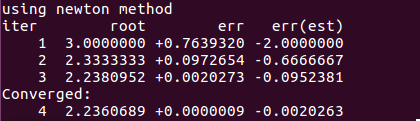
\includegraphics[width=1\linewidth]{images/newton.png}
				%\caption{newton}
			\end{figure}
				\begin{figure}[ht]
					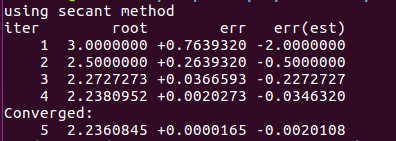
\includegraphics[width=1\linewidth]{images/secant.png}
				%	\caption{secant}
				\end{figure}
				\paragraph{}由图像可得,牛顿法与secant法相对于二分法,收敛性更强,收敛速度更快,所得解精度更高。
	\section{数值算例}
	下用牛顿法实现不同式子的求解。求解时应选取合适的初始近似解。
	
	\paragraph{Example1:}求解$2x^2+4x-3=0$
	\begin{figure}[ht]
		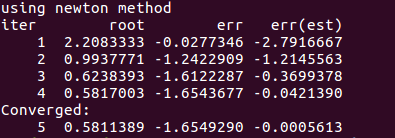
\includegraphics[width=1\linewidth]{images/n2.png}
		\caption{$2x^2+4x-3=0$}
	\end{figure}
	\paragraph{Example2:}求解$x^2+5=0$ \\
	选取不当的初始估计解会造成无法求解:
	\begin{figure}[ht]

		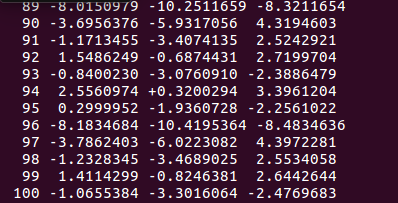
\includegraphics[width=1\linewidth]{images/n3.png}
		\caption{$x^2+5=0$}
	\end{figure}
	\section{结论} 
	利用二分法、牛顿法、Brent法等我们可以实现对一维非线性方程的求解。在求解过程中需主意选取合适的解区间或初始近似解。同时,给定同一方程时,不同的方法对应不同的迭代速度,我们可以结合给定方程的性质,选取合适的方法进行求解,从而获得更高的效率与更精确的结果。
	\bibliography{ref}
	\bibliographystyle{IEEEtran}
\end{document}
